\chapter{Planificación y estimación de costes}
\section{Planificación}

Este proyecto se ha estructurado en distintas fases, algunas de las cuales se han desarrollado de forma secuencial y otras en paralelo. La temporización se ha implementado mediante la aplicación GanttProject de código abierto y que se puede encontrar en \cite{GP}.
\bigskip
Las fases en las que se divide el desarrollo del proyecto son:

\begin{itemize}
\item \textbf{Fase 1:}Introducción teórica
	\begin{itemize}
	\item Lectura de la bibliografía.
	\item Clases sobre EDA.
	\item Hito tema 2.
	\item Hito tema 3.
	\item Hito tema 4.
	\end{itemize}
\item \textbf{Fase 2:}Documentación
	\begin{itemize}
	\item Explicación documentada de cada uno de los temas.
	\end{itemize}
	\item \textbf{Fase 3:}Análisis, diseño y desarrollo de la aplicación.
	\begin{itemize}
	\item Hito tema 7.
	\item Hito tema 8.
	\item Hito tema 9.
	\end{itemize}
	\item \textbf{Fase 4:}Caso de estudio.
	\begin{itemize}
	\item Hito tema 10.
	\end{itemize}
	\item \textbf{Fase 5:}Conclusiones.
	\begin{itemize}
	\item Hito tema 11.
	\end{itemize}
	\item \textbf{Fase 6:}Maquetación del documento final.
	\begin{itemize}
	\item Inclusión de todos los temas en un documento conjunto.
	\end{itemize}
\end{itemize}


\begin{landscape}
\begin{figure}
\centering
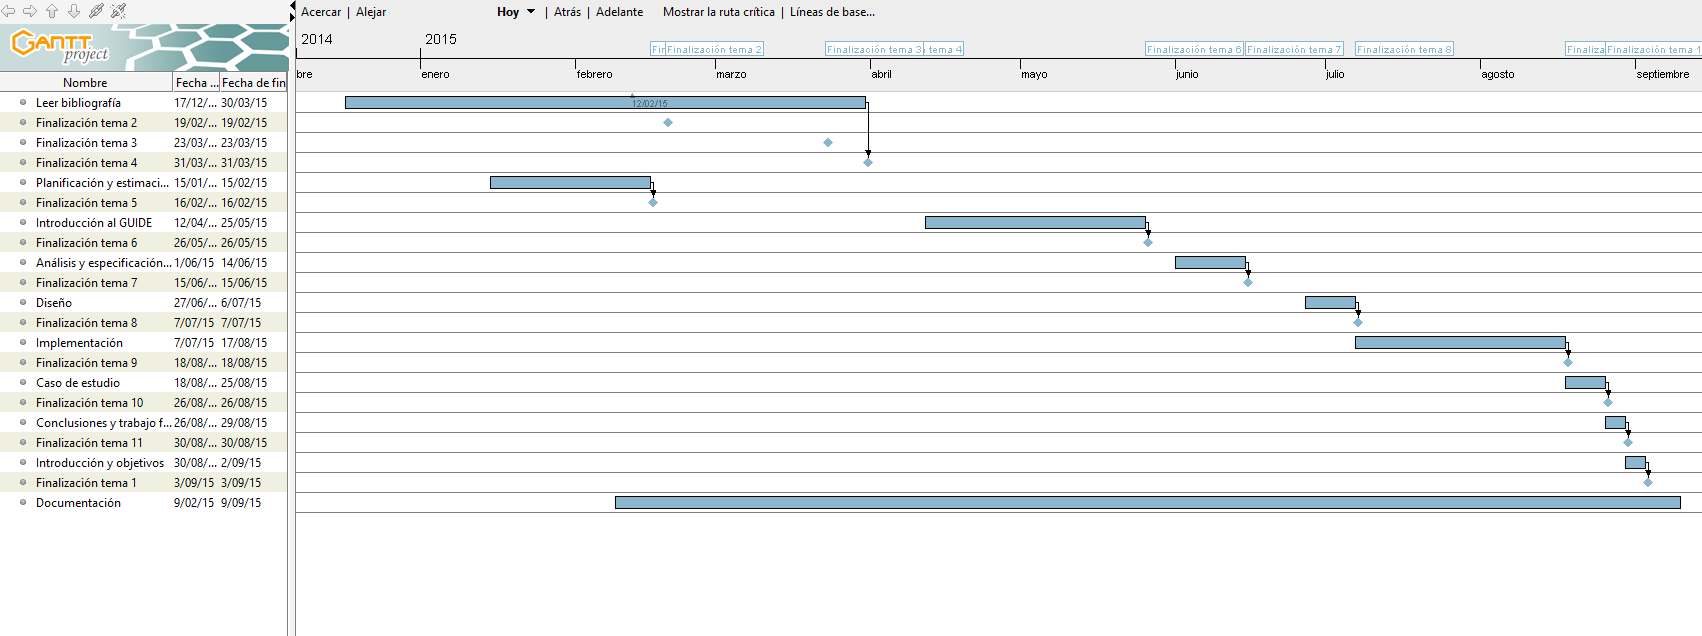
\includegraphics[width=1.8\textwidth]{imagenes/figuras/5_1.png}
\caption{Temporización en GanttProject.}
\end{figure}
\end{landscape}

\bigskip

Como se puede apreciar en la figura 5.1 la fase de documentación se hace en paralelo a cada una de las demás, puesto que el desarrollo de cada uno de los temas se van incluyendo en el documento final de forma progresiva.
Una estimación de las horas de trabajo dedicadas a cada fase aparece en la siguiente  tabla:

\bigskip
\begin{table}[htb]
\begin{center}
\begin{tabular}{|l|l|l|l|}
\hline
  & Días & Horas & Total \\
\hline \hline
Fase 1 & 104 & 2 & 208 \\ \hline
Fase 2 & 205 & 2 & 410 \\ \hline
Fase 3 & 66 &4 & 264 \\ \hline
Fase 4 & 8 & 6 & 40 \\ \hline
Fase 5 & 4 & 3 & 12 \\ \hline
Fase 6 & 6 & 6 & 36 \\ \hline
&&Tiempo total & 970 \\ \hline
\end{tabular}
\caption{Cálculo de horas de trabajo.}
\end{center}
\end{table}

\begin{figure}[H]
\centering
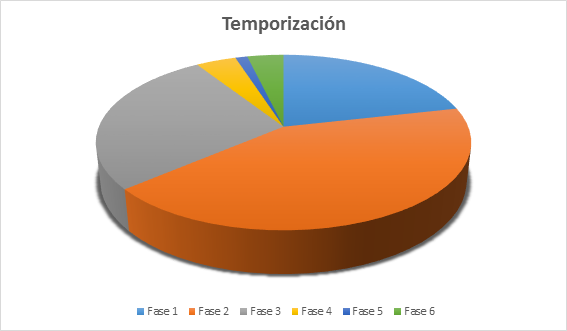
\includegraphics[width=0.9\textwidth]{imagenes/figuras/5_2.png}
\caption{Gráfico de la temporización.}
\end{figure}


\section{Recursos}
\subsection{Recursos humanos}

\begin{itemize}
\item D. José Camacho Páez, Profesor titular del departamento de Teoría de la señal, Telemática y comunaciones (TSTC) de la Universidad de Granada. Tutor del trabajo.
\item	Pablo Sánchez Robles, alumno de la Escuelta Técnica Superior de Ingeniería Informática y Telecomunicaciones (ETSIIT) de la Universidad de Granada. Autor del trabajo.
\end{itemize}
\bigskip
\subsection{Recursos hardware}
\begin{itemize}
\item Ordenador personal.
\end{itemize}

\bigskip

\subsection{Recursos software}

\begin{itemize}
\item Sistema operativo Windows 8.1.
\item Matlab® R2015a versión 8.5.
\item MEDA-Toolbox.
\item Evolus Pencil 2.0.5 (Diseño de interfaces gráficas)
\item ArgoUML 1.4	(Desarrollo de diagramas)
\item GanttProject 2.7.1	(Gráfico de temporización)
\item Texmaker	(Editor Latex)
\end{itemize}

\section{Estimación de costes}
\subsection{Herramientas hardware y software}
\begin{table}[htb]
\begin{center}
\begin{tabular}{|l|l|}
\hline
Recursos & Costes(Euros) \\
\hline \hline
Licencia Windows 8.1 & 138 \\ \hline
Matlab®(Student Version + toolboxes) & 321 \\ \hline
MEDA-Toolbox & 0 \\ \hline
Evolus Pencil & 0 \\ \hline
ArgoUML & 0 \\ \hline
GanttProject & 0 \\ \hline
Texmaker & 0 \\ \hline
Ordenador personal & 1200 \\ \hline
Total & 1659 \\ \hline
\end{tabular}
\caption{Costes herramientas.}
\end{center}
\end{table}

\bigskip
\begin{figure}[H]
\centering
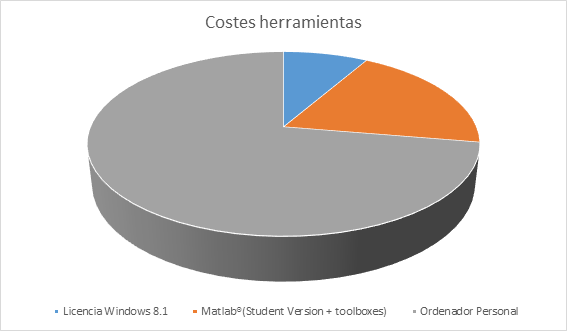
\includegraphics[width=0.9\textwidth]{imagenes/figuras/5_3.png}
\caption{Gráfico costes herramientas.}
\end{figure}
\bigskip

\subsection{Presupuesto}
Para el coste de los recursos humanos se ha hecho una estimación de 20 euros por hora trabajada por parte de Pablo Sánchez Robles y el coste del trabajo del tutor a 60 euros por hora, con una estimación de unas 50 horas de trabajo.

\bigskip

\begin{table}[htb]
\begin{center}
\begin{tabular}{|l|l|}
\hline
Concepto & Coste(Euros) \\
\hline \hline
Recursos humanos & 22400 \\ \hline
Herramientas & 1659 \\ \hline
Total & 24059 \\ \hline
\end{tabular}
\caption{Costes herramientas.}
\end{center}
\end{table}

\begin{figure}
\centering
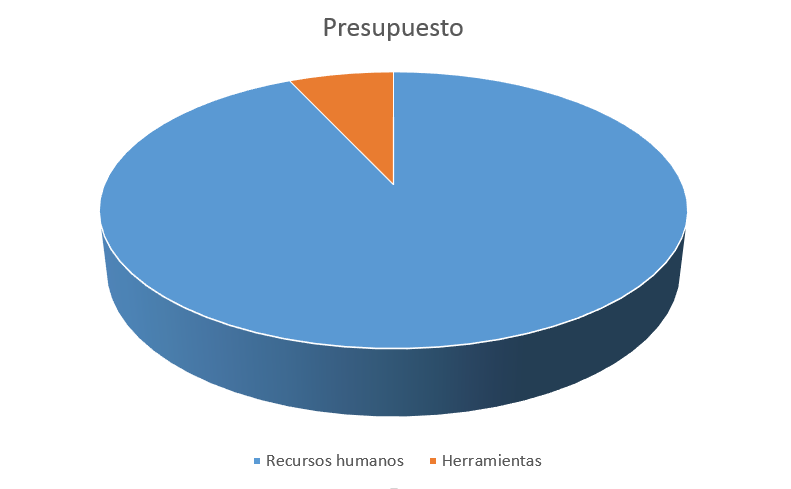
\includegraphics[width=0.9\textwidth]{imagenes/figuras/5_4.png}
\caption{Gráfico presupuesto total.}
\end{figure}
